%%%--------------------------------%%%
%%% UC11
%%%--------------------------------%%%

\newpage
% UC11 ====================================================
\subsubsection{Use Case Specification: \ac{UC}11 Progress Indicator}
\label{sec:domainBbl}

\paragraph*{Description}\mbox{}\\
This \ac{UC} deals with the user's journey through the application. 
It can be divided into three phases:
\begin{enumerate}
	\vspace{-3mm}
	\setlength\itemsep{-1em}
	
	\item Onboarding
	\item Scaffolding
	\item Progress
\end{enumerate}
\noindent
The \ac{UC}'s aim is to adapt the application to the different needs of the user in each phase.

\paragraph*{Screenshots}\mbox{}\\
tbd: Insert screenshots and shortly explain what can be seen
\begin{figure}[h] 
	\centering
	
\includegraphics[width=0.1\textwidth]{Content/Domain/placeholder.png}
	\caption{Use Case X: Detail}
	\label{fig:label8}
\end{figure}

\paragraph*{Basic Flow} \mbox{}\\

\begin{enumerate}
	\vspace{-3mm}
	\setlength\itemsep{-1em}
	
	\item Onboarding
	\begin{itemize}
		\vspace{-3mm}
		\setlength\itemsep{-1em}
		
		\item The user has registered and logs in for the first time.
		\item A welcome dialog is displayed. It contains some minimal information about the application. At the end of this dialog there's a list of activities which can be done next by the user. The list of possible activities should be adapted dynamically to the user's status (e.g. already member of a project or not).
	\end{itemize}

	\item Scaffolding
	\begin{itemize}
		\vspace{-3mm}
		\setlength\itemsep{-1em}
		
		\item Info boxes providing help about the usage and behavior of the application.
		\item Progress bar, displaying and motivating new tasks which can be done by the user next.
	\end{itemize}

	\item Progress
	\begin{itemize}
		\vspace{-3mm}
		\setlength\itemsep{-1em}
		
		
		\item The reached badges are displayed prominently at the start page and on the user detail page. The conception of badges in detail is described in TODO: ref auf gamification conception \ref{TODO}.
		\item The user is rewarded for desired behavior by points, which represent an activity indicator for each user. This is visualized for the user by a chart of reached points over time.
	\end{itemize}
\end{enumerate}

\subparagraph{Activity Diagram}\mbox{}\\
\begin{figure}[H]
	\centering
	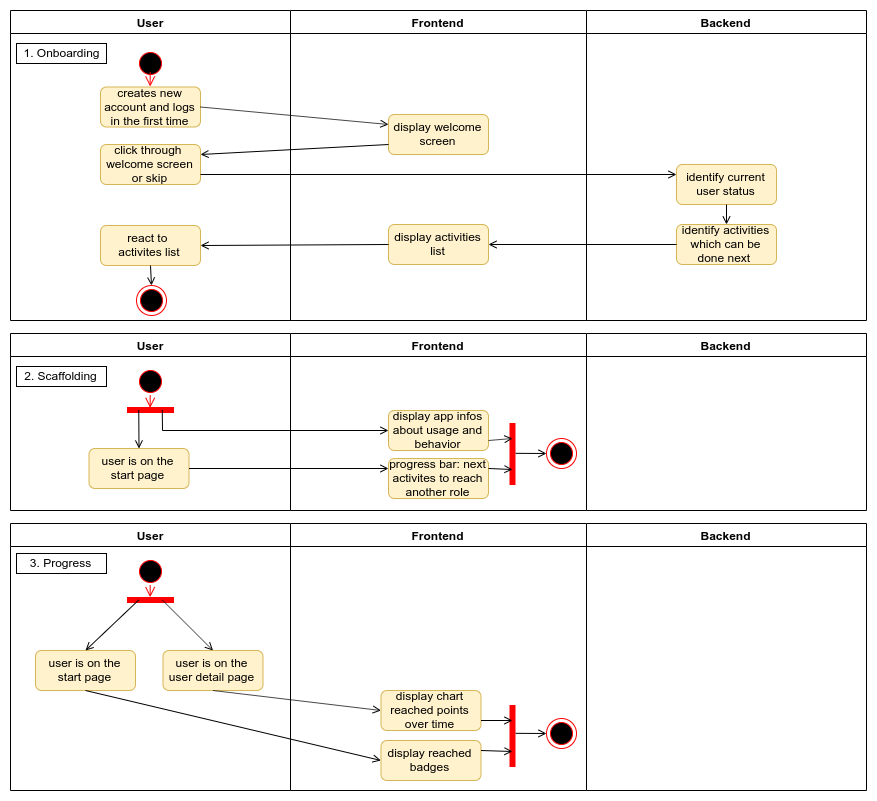
\includegraphics[width=1.0\textwidth]{Content/Domain/UC11ProgressIndicator.png}
	\caption{Activity Diagram  \ac{UC}11 Progress Indicator}
	\label{fig:label12}
\end{figure}

\paragraph*{Alternative Flows}\mbox{}\\
N/A

\paragraph*{Special Requirements and Preconditions}\mbox{}\\
As a precondition the user has to create an account and login for the first time. 

\paragraph*{Postconditions and Persistance}\mbox{}\\
The user was accompanied from beginner to an expert user. Therefore as a postcondition the user is advanced in using the application.

\newpage